\documentclass{article}
\usepackage{v-problem}
\vgeometry

\begin{document}
\vtitle[ROTATION]

\def\pn{02}
\def\book{A.K.}
\def\page{40}
\def\gdrive{https://drive.google.com/drive/folders/1tsHmVHqpBEMud9Gvzqlwrzm9OkD4FR6S?usp=share_link}

\def\question{
A homogeneous sphere of radius $r$ rolls without slipping with constant angular speed $\omega'$ over bigger sphere, of radius $R$, which is in pure rotation with constant angular speed $\omega$ about its centre $O$. (Fig.)
Find the time taken for the point of contact of the rolling
sphere to make one full revolution over
the bigger rotating sphere.
}

\vspace*{\fill}
\begin{tikzpicture}
	\node[qnumber] (n) at (0, 0)[scale=2] {$\pn.$};
	\node[question] (q) [right=2mm of n.east] {\question};
	\tzline[divider]<-0.125, 0> (q.north west)(q.south west);
	\node[format] (f) at  (q.south east){[\book \quad \page]};
\end{tikzpicture}	
\vspace*{\fill}

\begin{center}
\begin{tikzpicture}
[thick]
\def\R{1.5}
\def\r{1}
\tzcoor*(0,  0)(O){$O$}[b]
\tzcoor*(45:\R+\r)(C){$C$}[r]
	\tzcircle(O)(\R)
	\tzline[->](O)(-120:\R){$R$}[ml]
	\tzcircle(C)(\r)
	\tzarc[->](O)(100:190:\R+0.4){$\omega$}[ma]
	\tzarc[->](C)(60:120:\r+0.35){$\omega'$}[ma]
	\tzline+[->](C)(60:\r){$r$}[ml]
	\tzline[dashed](0, 0)(45:\R+\r)
\end{tikzpicture}
\end{center}

\pagebreak

\vspace*{\fill}
\begin{center}
	\fbox{\qrcode[height=2cm]{\gdrive}}
\end{center}
\vspace*{\fill}

\end{document}
